The national estimates in \citet{biasi_what_2025} summarize the \emph{average} effect of school capital investments, but a national average is only as portable as the effects underlying it are similar. A growing literature shows that design-based estimates of school-spending effects vary widely across settings \citep{jackson2024impacts,handel2024contexts}, and that an average estimated from the contexts that happen to enter a study need not describe the policy's return elsewhere \citep{allcott2015site}. Because a stacked dynamic design recovers a precision-weighted aggregate of underlying cohort- and state-specific effects \citep{goodmanbacon2021difference,sunabraham2021estimating,callaway2021difference}, decomposing that aggregate is the natural way to gauge how far the national result generalizes. I therefore re-estimate the stacked dynamic RD specification separately for each state with sufficient usable data, using the same event-time windows as the main replication: years 1--5, 6--8, and 9--10 for capital spending, and years 1--4, 5--8, and 9--12 for test scores and house prices. Because per-state estimates are individually noisy, I read the collection of state effects as a \emph{distribution} of returns rather than as a ranking of states, in the spirit of the hierarchical treatment of heterogeneous estimates in \citet{meager2019understanding,meager2022aggregating}. Figure \ref{fig:state_forest} collects the state-specific estimates for all three outcomes.

\subsection{Capital Spending}

Panel (A) of Figure \ref{fig:state_forest} shows that bond authorization does not translate into identical capital-spending responses across states. Several states show large short-run increases in capital expenditures per pupil, while others show smaller or imprecise responses. This heterogeneity matters for interpretation: later test-score and housing-price effects are mediated by whether authorized bonds actually generate new capital investment and by the timing of that spending.

\subsection{Test Scores}

Panel (B) of Figure \ref{fig:state_forest} reports state-specific reduced-form effects on standardized test scores, and it is the central piece of evidence on external validity. The confirmed national effect is positive, but the state-level estimates are spread on both sides of it: a number of states show positive medium- or long-run effects, while others are near zero or negative, and the dispersion across states is large relative to the national point estimate. Two states can therefore both be consistent with the national average while implying very different local returns to a capital project. This is the same lesson \citet{cummins2017heterogeneous} draws in revisiting an influential education experiment---an informative average can coexist with subgroups for which the effect is small or reversed---and it is the quantitative content of the ``contexts of convenience'' caution of \citet{handel2024contexts}: the national estimate describes the policy's return in the average reporting state, not in any particular one. Consistent with the meta-analytic evidence on school spending \citep{jackson2024impacts}, the message is not that the original average is wrong, but that it should be used as a distribution of plausible state-level returns rather than as a single transportable number.

\subsection{Housing Market Responses}

Panel (C) of Figure \ref{fig:state_forest} shows a similarly heterogeneous pattern for housing prices. In some states, house prices rise after bond authorization, consistent with capitalization of expected improvements in school quality or local amenities. In other states, the estimates are small, negative, or imprecise. These patterns are consistent with the possibility that housing-market responses depend on both the perceived benefits of capital projects and the fiscal costs associated with bond repayment.

\begin{figure}[p]
    \centering
    \renewcommand{\thesubfigure}{\Alph{subfigure}}
    \begin{subfigure}{0.59\textwidth}
        \centering
        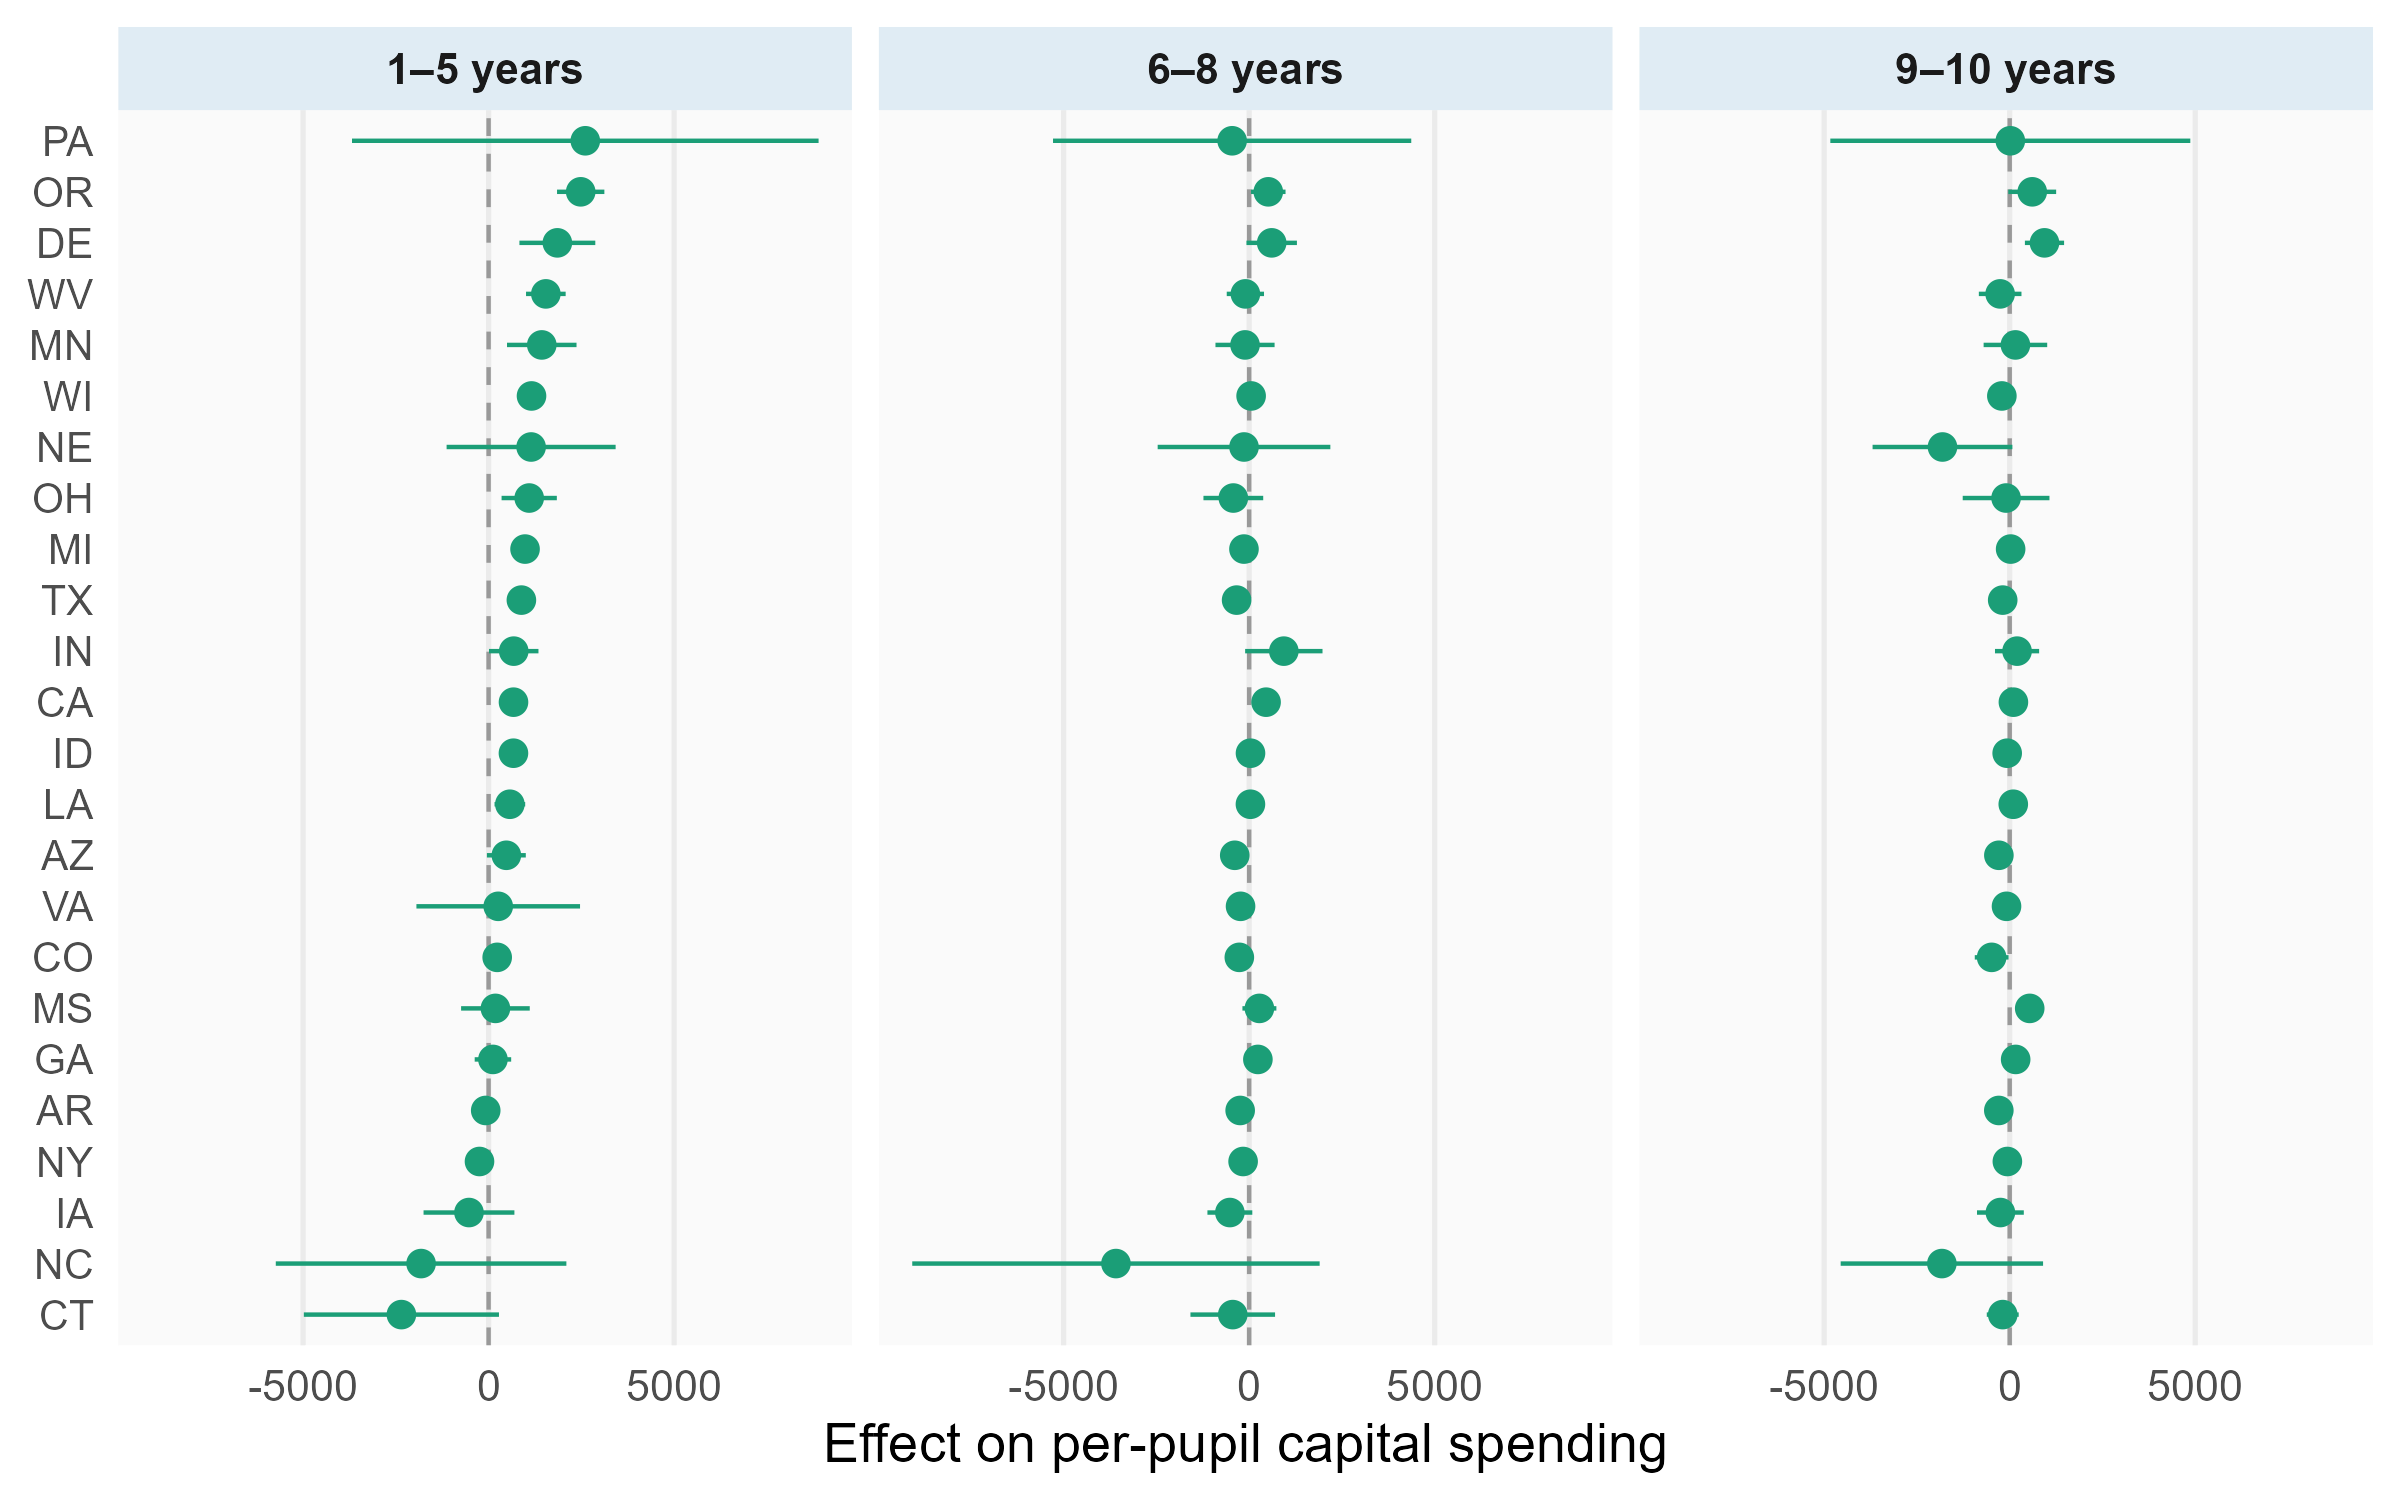
\includegraphics[width=\textwidth]{images/forest_capital.png}
        \caption{Capital expenditures per pupil}
        \label{fig:capital_forest}
    \end{subfigure}

    \vspace{0.2em}
    \begin{subfigure}{0.59\textwidth}
        \centering
        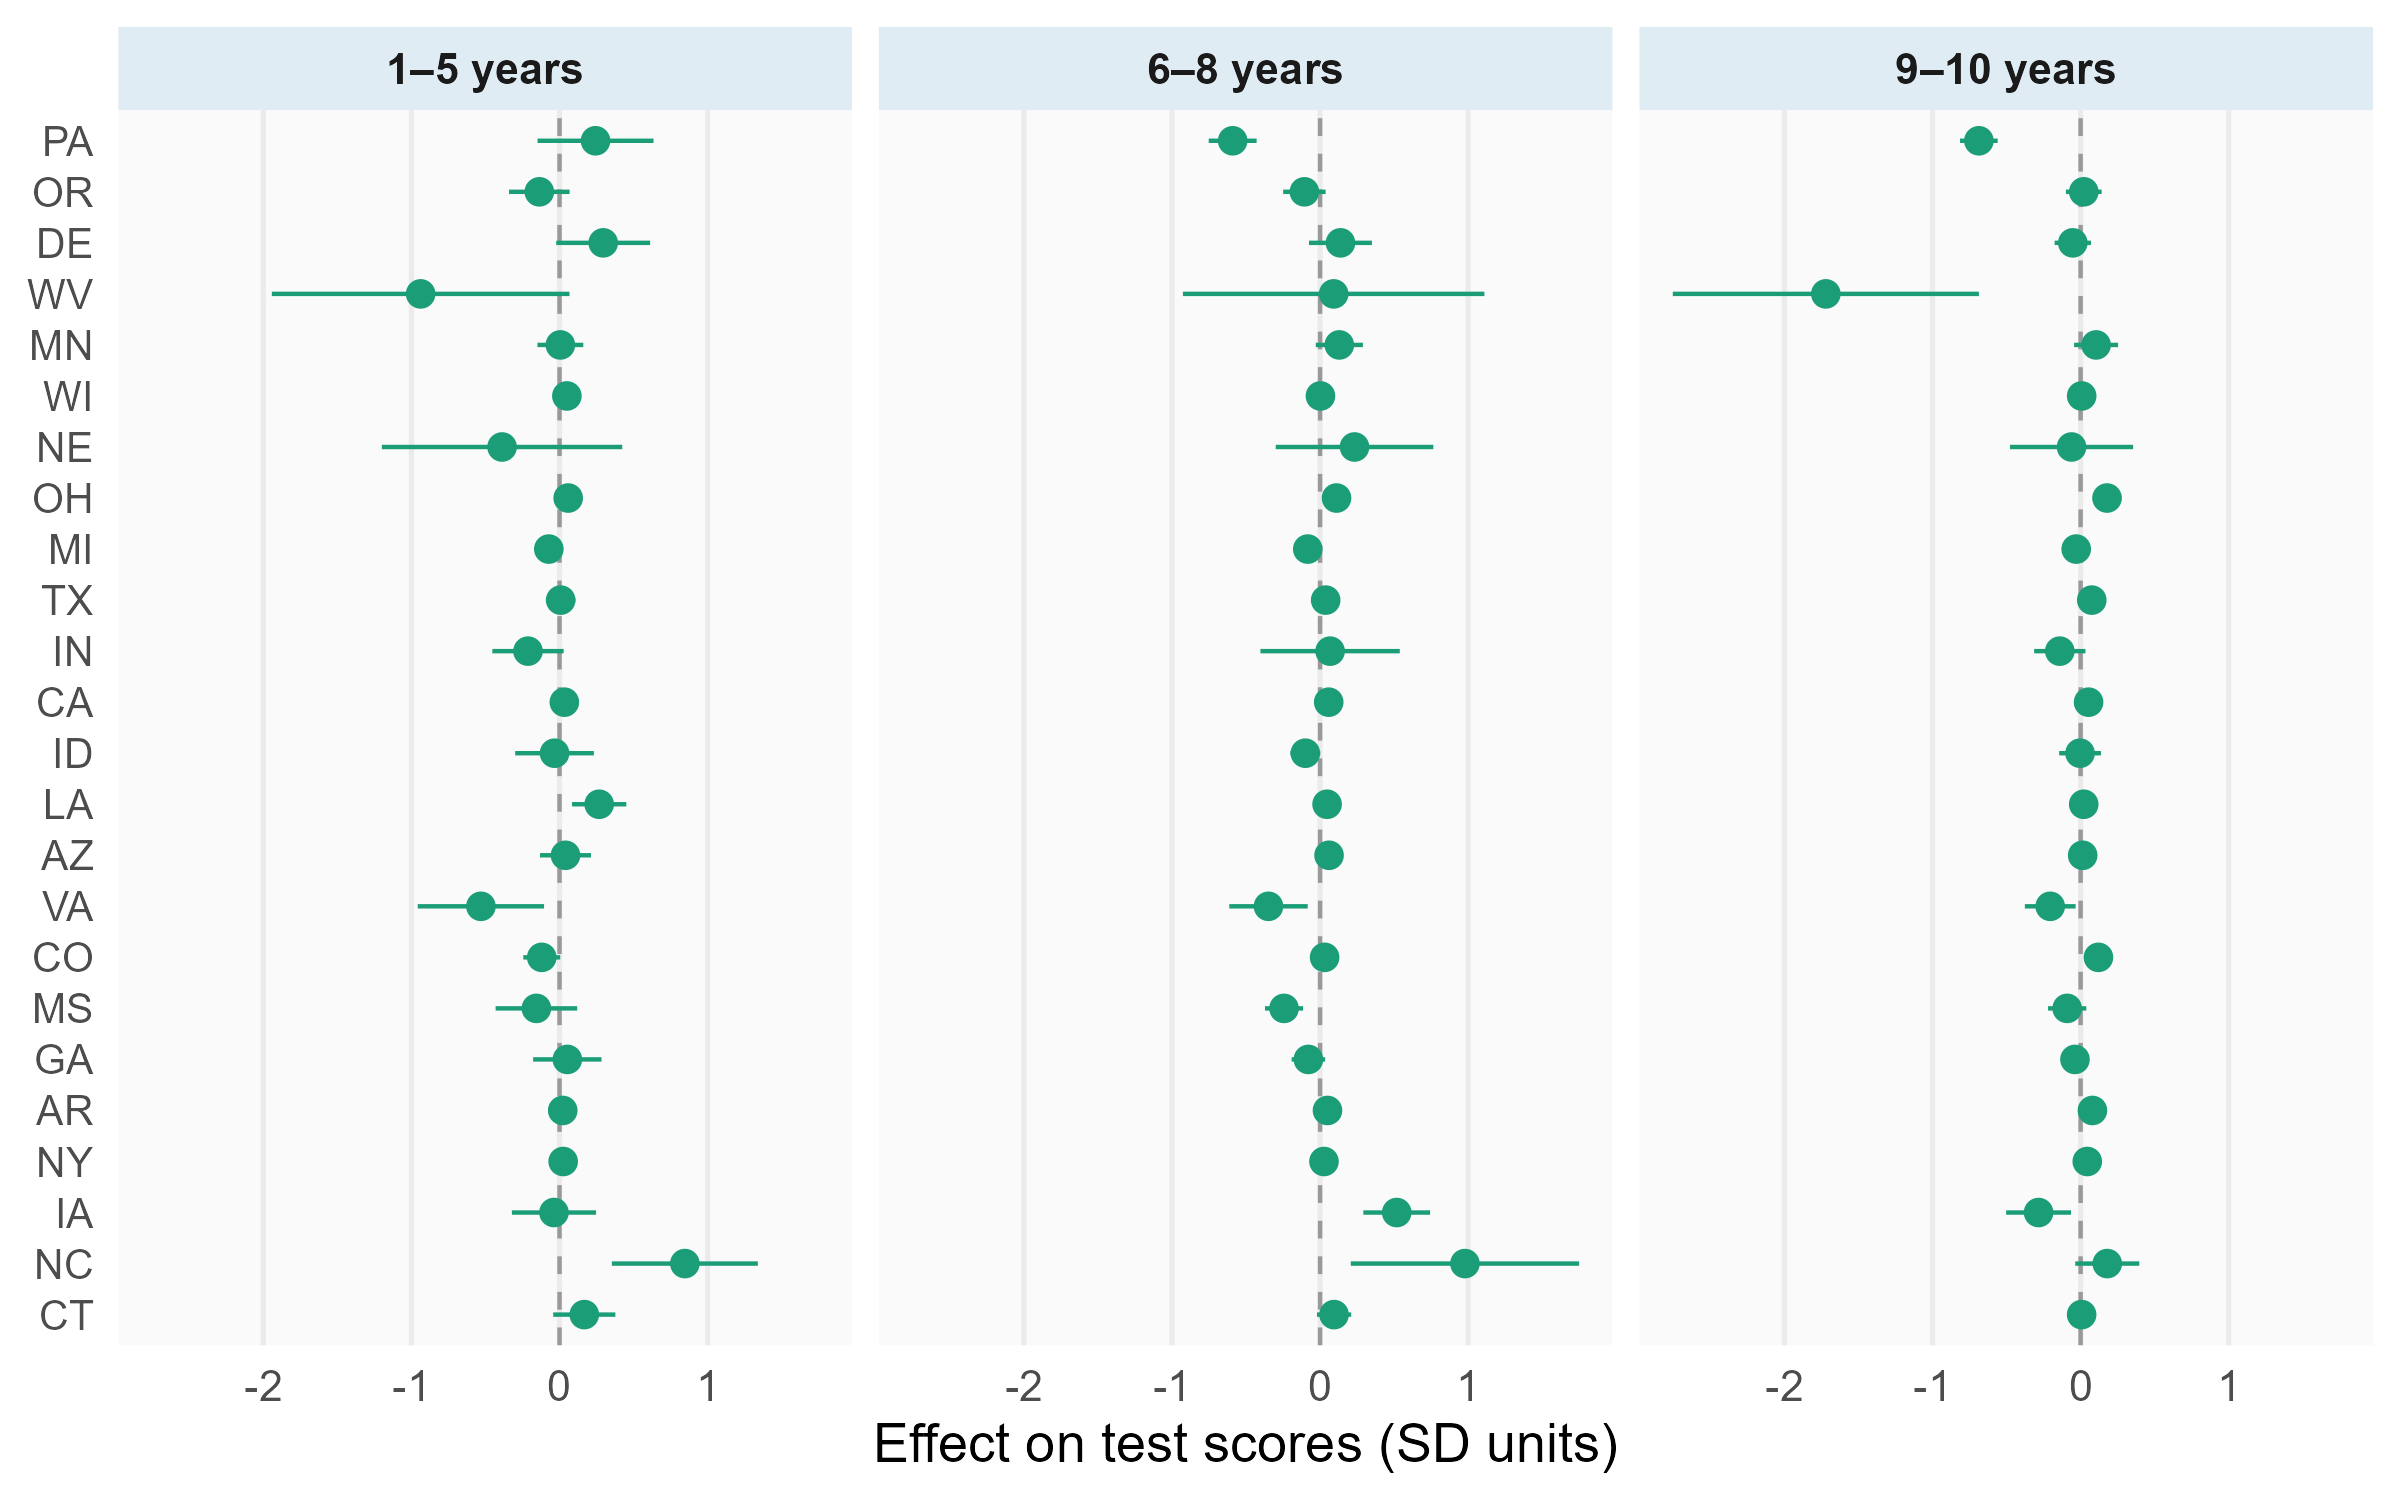
\includegraphics[width=\textwidth]{images/forest_tests.png}
        \caption{Test scores}
        \label{fig:tests_forest}
    \end{subfigure}

    \vspace{0.2em}
    \begin{subfigure}{0.59\textwidth}
        \centering
        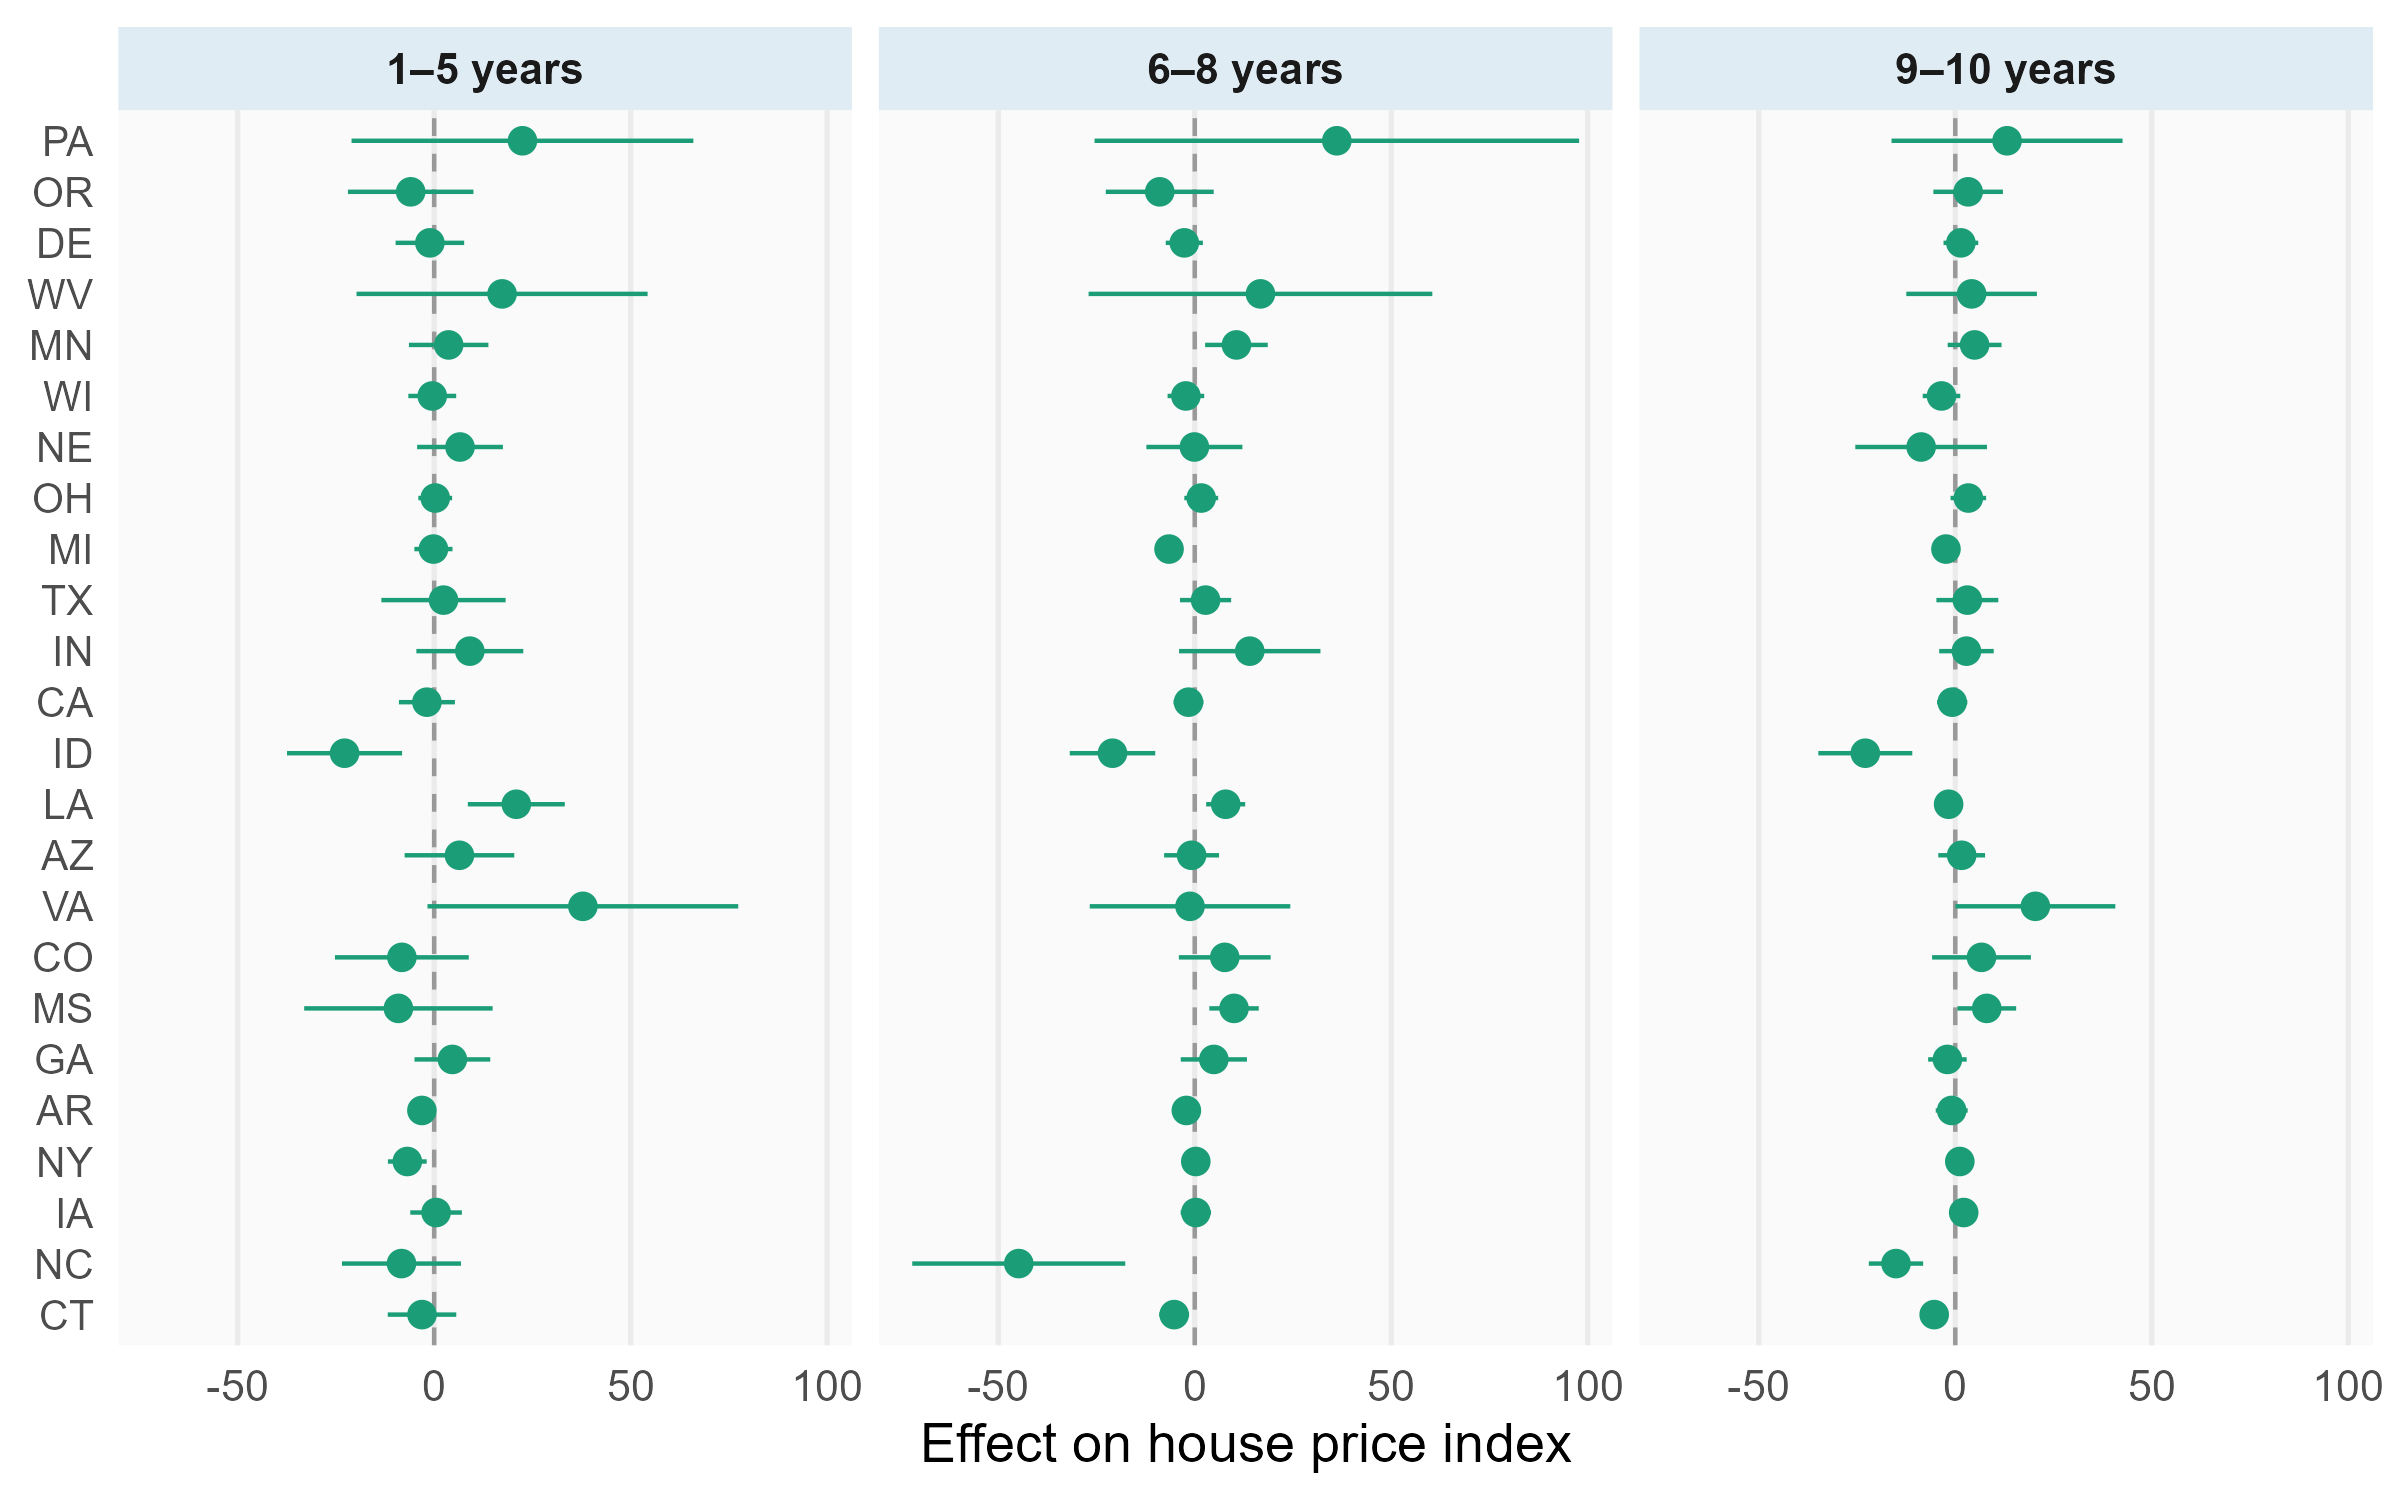
\includegraphics[width=\textwidth]{images/forest_hpi.png}
        \caption{House price index}
        \label{fig:hpi_forest}
    \end{subfigure}
    \caption{Effect of School Bond Authorization by State}
    \label{fig:state_forest}
    \captionsetup{font=footnotesize}
    \caption*{\footnotesize\textit{Notes:} Markers are state-specific stacked dynamic RD point estimates and whiskers are district-clustered confidence intervals; underlying values and exact event-time horizons appear in Appendix Tables \ref{tab:state_capital}--\ref{tab:state_house_prices}.}
\end{figure}

\subsection{Descriptive Mechanism Evidence}

A natural next question is whether the cross-state dispersion lines up with the mechanisms emphasized by \citet{biasi_what_2025}: the type of capital project, the quality of the pre-existing capital stock, and the characteristics of students served. I link the state-level estimates to descriptive state averages from the replication package---project-category shares, baseline capital stock, free or reduced-price lunch share, and minority share---while stressing that these variables are correlates, not causal instruments, for state heterogeneity, since states are few and were not randomly assigned their project mix or demographics \citep{allcott2015site}.

Appendix Figure \ref{fig:state_mech} plots the medium-run test-score effects against these mechanism variables, and the appendix tables report the underlying summaries and bivariate associations. The associations are weak and imprecise: with roughly two dozen noisy state estimates and incomplete project-category coverage, the data cannot adjudicate among the candidate mechanisms. I therefore treat them as hypothesis-generating rather than as confirmatory evidence on the mechanisms. Their value is to identify which contexts---project types, capital-stock conditions, and student populations---most warrant the properly powered, design-based mechanism analysis that would be needed to explain why the return to capital investment generalizes well to some states and not others, the kind of work that \citet{handel2024contexts} argue the school-finance literature most needs.
